\documentclass{DOEproposal}
%%%%%%%%%%%%%%%%%%%%%%%%%%%%%%%%%%%%%%%%%%%%%%%%%%%%%%%%%%%%%%%%%%%%%%%%%%%%%%%
% NSF proposal generation template style file.
% based on latex stylefiles  written by Stefan Llewellyn Smith and
% Sarah Gille, with contributions from other collaborators.
%
% Additions by Ronni Grapenthin, New Mexico Tech.
%
% Obviously it is your responsibility to make sure that everything
% is, in fact, in agreement with the most current NSF Grant 
% Proposal Guide and the respective Program's solicitation! 
% This is all provided `as-is' and no blame or responsibility
% for anything that went wrong will be taken.
%
% Good luck!
%
%%%%%%%%%%%%%%%%%%%%%%%%%%%%%%%%%%%%%%%%%%%%%%%%%%%%%%%%%%%%%%%%%%%%%%%%%%%%%%%

\usepackage{amsmath, amsthm, amssymb}
\usepackage{latexsym}
\usepackage{epsfig}
\usepackage{epstopdf}
\usepackage{graphicx}
\usepackage[footnotesize,bf]{caption}
\usepackage[final]{pdfpages}
\usepackage{hyperref}
\hypersetup{
    colorlinks=true,        % false: boxed links; true: colored links
    linkcolor=blue,         % color of internal links
    citecolor=black,        % color of links to bibliography
    filecolor=magenta,      % color of file links
    urlcolor=magenta,       % color of external links
    pdfstartview=           % omit this key from pdf dictionary so reader 
}                           %     just uses user default


% ----------------------------------
% Things to remove!
% ----------------------------------
% Add line numbers to draft
\usepackage{lineno}
\linenumbers
% Lorem ipsum generator for template
\usepackage{lipsum}
% Some definition to make collab. 
% editing easier. 
% ================================================
% Assign each person a color for in=text comments.
% ================================================
\usepackage[dvipsnames]{xcolor}
% For a list of named colors, see:
%     https://en.wikibooks.org/wiki/LaTeX/Colors#The_68_standard_colors_known_to_dvips

% --------------------------------------------------------------------------
% These definitions define a \NAME command which, when used like:
%    \NAME{Some comment.}
% will produce:
%    NAME says:  Some commnet.
% in the generated PDF. The comment will also be colored with NAME's color. 
% --------------------------------------------------------------------------
% A cool person 
\newcommand{\cool}[1]{{\color{Red}Cool says:~#1}}


% ----------------------------------


% Use roman numerals to number all pages before the narrative.
\pagenumbering{roman}

% The PI's information
\investigator{A really cool person}
\institute{Oak Ridge National Laboratory}
\phone{907-867-5309}
\email{cool@person.org}

% setup the title page.
% NOTE: you'll have to edit the imported file.
\title{A really good title}
\date{May 19, 2016}
\renewcommand*{\maketitle}{\begin{titlepage}
    \begin{center}
        { \Large \bf \Title }
        
        \vspace{1em}
        A proposal submitted to the DOE Office of Science \\
        \Date \\
        
        \vspace{1em}
        \emph{Invited Proposal:} CMDV-SE Activity \\                                                                          
        \emph{DOE Office of Science Program Manager:} Dorothy Koch \\
        
        \vspace{1em}
        \begin{table}[h!]                                                                                         
            \centering
            \begin{tabular}{ l l }                                                                                   
                \emph{Proposing Organization:}  &  \Institute \\[1em]
                
                \emph{Collaborating Institutions:} & Lawrence Livermore National Laboratory \\
                & Pacific Northwest National Laboratory  \\
                & Sandia National Laboratories  \\[1em]

                \emph{Principal Investigator:}  & \Investigator \\         
                & Computer Science and Mathematics Division \\ 
                & PO Box 2008, Mail Stop 6301 \\  
                & Oak Ridge, TN 37831-6301 \\ 
                & Phone: \Phone \\ 
                & Email: \Email \\[1em]

                \emph{Requested Funding:} & {\$1.5M/year for three years} \\
                \emph{Total Request:}     & {\$4.5M}   \\
            \end{tabular}
        \end{table}
    
        \vspace{1em}
        Budget Summary: \\
        \vspace{0.5em}
        \begin{tabular}{|l|r|r|r|}                                                                                   
            \hline
            {\bf Institution} & {\bf Year 1} & {\bf Year 2} & {\bf Year 3} \\
            \hline
            Oak Ridge National Laboratory & \$500K & \$500K & \$500K \\ \hline
            Pacific Northwest National Laboratory & \$500K & \$500K & \$500K \\ \hline
            Sandia National Laboratories   & \$500K & \$500K & \$500K \\ \hline
        \end{tabular}
    \end{center}
\end{titlepage}                                                                                                         

}

% set the bibliography style
%\bibliographystyle{ametsoc2014}
\bibliographystyle{agufull08}

%%%%%%%%%%%%%%%%%%%%%%%%%%%%%%%%%%%%%%%%%%%%%%%%%%%%%%%%%%%%%%%%%%%%%%%%%%%%%%%
% Begin the document
%%%%%%%%%%%%%%%%%%%%%%%%%%%%%%%%%%%%%%%%%%%%%%%%%%%%%%%%%%%%%%%%%%%%%%%%%%%%%%%
\begin{document}
    % make the title page
    \maketitle

    % make the table of contents
    \renewcommand{\contentsname}{Table of Contents}
    \tableofcontents
    \newpage

    % the abstract
    \begin{center}
        {\bf \Large Abstract}
    \end{center}
    \addcontentsline{toc}{section}{Abstract}
    \noindent
{\bf Title:} \Title

\vspace{0.5em}
\noindent
{\bf Lead Institution:} \Institute

\vspace{0.5em}
\noindent
{\bf Principal Investigator:} \Investigator


\vspace{0.5em}
\noindent
{\bf Co-Investigator:}  This Person (Deputy-PI; LLNL PI) Person 0, Person 9 (LLNL);
                        That Person (PNNL PI), Person 1, Person 2 (PNNL);
                        Another Person (SNL PI) Person 3, Person 4 (SNL);
                        Differnt Person (UAF)


\vspace{0.5em}
\noindent
%FIXME: Put your text here!
\lipsum[1-4]


    \newpage

    % setup the main body of the proposal
    \pagenumbering{arabic}
    \addcontentsline{toc}{section}{Proposal Narrative}
    \setcounter{page}{1}

    
    % the main body of the proposal
    \noindent

% Section 1
\section{Introduction}
    \label{sec:introduction}
    \lipsum[5]


    \vspace{0.5em}
    \subsection{Motivation}
        \label{sec:motivation}
        \lipsum[6-7]

\vspace{0.5em}
\noindent
{\bf Theme 1: An overarching theme.}
\lipsum[8]
{Blah blah blah all support Theme 1.}

\vspace{0.5em}
\noindent
{\bf Theme 2: Another overarching theme.}
\lipsum[9]
{Blah blah blah all support Theme 2.}

\vspace{0.5em}
\noindent
{\bf Theme 3: Final overarching theme.}
\lipsum[10]
{Blah blah blah all support Theme 3.}

Our definition of sucess\ldots
\begin{itemize}
    \item This thing will be done.
    \item So will this.
    \item Oh and this to.
\end{itemize}


    \vspace{0.5em}
    \subsection{Background}
        \label{sec:background}
        \lipsum[11-20]


    \vspace{0.5em}
    \subsection{Selection of Tasks}
        \label{sec:selectedtasks}
        \lipsum[21-30]

In addition to the proposed work sections above, this proposal includes a
Management Plan (Section~\ref{sec:management}), a Data Management plan,
(Section~\ref{sec:data_management}), and a Software Productivity and
Sustainably Plan (Section {\ref{sec:software_sustainability}). In addition, we
have included supplemental materials of a Project Staffing Overview
(Section~\ref{sec:staffing}), a detailed timetable for deliverables and tasks
(Section~\ref{sec:timetable}), a list of abbreviations and code names
(Section~\ref{sec:abbreviations}, and short CVs for all key personnel.



% Section 2
\section{Proposed Research: Something Neat}
    \label{sec:neat}
    \lipsum[31-40]



    \vspace{0.5em}
    \subsection{Some details}
        \label{sec:somedetails}
        %FIXME: place this subsection in a file here:
        %\input{Text/SEC2/}
        \lipsum[41-50]

    \vspace{0.5em}
    \subsection{Other details}
        \label{sec:otherdetails}
        %FIXME: place this subsection in a file here:
        %\input{Text/SEC2/}
        \lipsum[51-60]


% Section 3
\section{Proposed Research: Something Else Neat}
    \label{sec:elseneat}
    \lipsum[61-70]



    \vspace{0.5em}
    \subsection{Set of details}
        \label{sec:setdetails}
        %FIXME: place this subsection in a file here:
        %\input{Text/SEC3/}
        \lipsum[71-80]

    \vspace{0.5em}
    \subsection{Anoth set of details}
        \label{sec:anotherdetails}
        %FIXME: place this subsection in a file here:
        %\input{Text/SEC3/}
        \lipsum[81-90]


% Continue adding sections to your hearts desire... 






    
    
    % Extras
    \section{Project Management Plan}
        \label{sec:management}
        \lipsum[91-100]


    \section{Data Management Plan}
        \label{sec:data_management}
        \lipsum[101-110]


    \section{Software Productivity and Sustainability Plan}
        \label{sec:software_sustainability}
        \lipsum[111-120]



    % end of proosal narrative
    %NOTE: 50 page limit is to here.
    \vspace{1em}
    \section*{\underline{End of proposal narrative; supplemental materials to follow.}}
    \newpage


    % supplemental materials
    \addcontentsline{toc}{section}{Supplemental Materials:}
    \section{Project Staffing Overview}
        \label{sec:staffing}
        \lipsum[121-130]

    \newpage

    \section{Project Timeline, Deliverables, and Tasks}
        \label{sec:timetable}
        \lipsum[131]
The targeted due dates for the deliverables are indicated in quarter year
increments: e.g., Q4 referes to delivery one year after the project funding
begins, and Q12 referes to the end of the three-year project.

%NOTE: Use enumerate to get the proper section heddings, then nested itemized
%lists to get major/minor tasks. This SHOULD match your table of contents.


%stuff to make enumerate mimic section numbering:
\renewcommand{\labelenumii}{\arabic{enumi}.\arabic{enumii}}
\renewcommand{\labelenumiii}{\arabic{enumi}.\arabic{enumii}.\arabic{enumiii}}
\renewcommand{\labelenumiv}{\arabic{enumi}.\arabic{enumii}.\arabic{enumiii}.\arabic{enumiv}}

\begin{enumerate}
\setcounter{enumi}{1} %start on sect 2 for consistency w/ section labeling.

    \item Something Neat
        \begin{enumerate}
            \item Some details
                \begin{itemize}
                    \item Major task 1 (Q6)
                        \begin{itemize}
                            \item Minor Task 1 (Q2)
                            \item Minor Task 2 (Q4)
                            \item Minor Task 3 (Q6)
                        \end{itemize}
                    \item Major task 2 (Q8)
                        \begin{itemize}
                            \item Minor Task 4 (Q3)
                            \item Minor Task 5 (Q6)
                            \item Minor Task 6 (Q8)
                        \end{itemize}
                \end{itemize}
        \end{enumerate}
        \begin{enumerate}
            \item Other details
                \begin{itemize}
                    \item Major task 3 (Q6)
                        \begin{itemize}
                            \item Minor Task 1 (Q2)
                            \item Minor Task 2 (Q4)
                            \item Minor Task 3 (Q6)
                        \end{itemize}
                    \item Major task 4 (Q8)
                        \begin{itemize}
                            \item Minor Task 4 (Q3)
                            \item Minor Task 5 (Q6)
                            \item Minor Task 6 (Q8)
                        \end{itemize}
                \end{itemize}
        \end{enumerate}

    \item Something Else Neat
        \begin{enumerate}
            \item Set of details
                \begin{itemize}
                    \item Major task 1 (Q6)
                        \begin{itemize}
                            \item Minor Task 1 (Q2)
                            \item Minor Task 2 (Q4)
                            \item Minor Task 3 (Q6)
                        \end{itemize}
                    \item Major task 2 (Q8)
                        \begin{itemize}
                            \item Minor Task 4 (Q3)
                            \item Minor Task 5 (Q6)
                            \item Minor Task 6 (Q8)
                        \end{itemize}
                \end{itemize}
        \end{enumerate}
        \begin{enumerate}
            \item Another set of details
                \begin{itemize}
                    \item Major task 3 (Q6)
                        \begin{itemize}
                            \item Minor Task 1 (Q2)
                            \item Minor Task 2 (Q4)
                            \item Minor Task 3 (Q6)
                        \end{itemize}
                    \item Major task 4 (Q12)
                        \begin{itemize}
                            \item Minor Task 4 (Q5)
                            \item Minor Task 5 (Q10)
                            \item Minor Task 6 (Q12)
                        \end{itemize}
                \end{itemize}
        \end{enumerate}

\end{enumerate}


    \newpage


    % The bibliography 
    \section{Abbreviations and Code Names}
        \label{sec:abbreviations}
        \begin{tabular}{p{1.0in}p{5.4in}}
    ACME & Accelerated Climate Model for Energy (both code and project) \\
    ACME v0 & Version 0.0 of ACME model, 2014 \\
    ACME v1 & Version 1.0 of ACME model, 2016 \\
    ACME v2 & Version 2.0 of ACME model, ~2018 \\
\end{tabular}

    \newpage

    \section{Literature Cited}
        \label{sec:references}
        \bibliography{main}
    \newpage
   

    % The short biosketches for EVERY contributing person
    \section{Biographical Sketches}
        \label{sec:biosketches}
        
The following pages list 2-page CVs for the key personnel listed below.

\begin{itemize} \zapspace
    \item{\Investigator}
    \item{This Person} 
    \item{Person 0} 
    \item{Person 9} 
    \item{That Person} 
    \item{Person 1} 
    \item{Person 2} 
    \item{Another Person} 
    \item{Person 3} 
    \item{Person 4} 
    \item{Different Person} 
\end{itemize}

\newpage

% NOTE: You can import tex bios like so
\newpage

\begin{center}
    {\Large\bf A Really Cool Person} \\[0.25em]
    Oak Ridge National Laboratory \\
    P.O. Box 2008, MS 6301 \\
    Oak Ridge, TN 37831 \\
    Email:cool@person.org
\end{center}

\noindent\textbf{Education and Training}

\vspace{1.5em}
\begin{tabular}{rp{5.6in}}
    2010 & Ph.D., Physics, Very Prestigious University, Big City, Little State \\[0.5em]
    2003 & B.S., Physics, Nice State School, Little City, Big State
\end{tabular}
\vspace{1.5em}
    
\noindent\textbf{Research and Professional Experience}

\vspace{1.5em}
\begin{tabular}{lp{5in}}
    {2015--present} & Postdoctoral research associate, Oak Ridge National Laboratory, Oak Ridge, TN. \\[0.5em]
    {2008--2015}    & Graduate research assistant, Very Prestigious University, Big City, Little State.
\end{tabular}

\vspace{1.5em}

\noindent\textbf{Selected Software Releases and Publications} % Top 10!

\begin{itemize}

\item[] Software: I am the lead developer of the Functional Othgraphic Olograph (FOO), which is a python-based, extensible verification and validation suite for Umpa Lumpas. Latest public, open-source release of FOO was version 2.0 on July 9, 2012.  



\item[] ``Super exciting title'',
        {\bf A Very Cool Person}, Other Person, and Another Person, 
        {\sl{Journal of Olography}}, {\bf 227}:537-550, (2015).
        \href{http://dx.doi.org/10.1029/2012JF002343}{doi:10.1029/2012JF002343}.
\end{itemize}

\noindent\textbf{Synergistic Activities} % 5!

\vspace{1.5em}
\begin{tabular}{lp{5.2in}}
    2015--present & Currently participating in the Functional Othgraphic Olograph Basic Aptitude Results Intercomparison Project 6 (FOOBAR-IP6). \\[0.5em] 

\end{tabular}
\vspace{1.5em}

\noindent\textbf{Collaborators}
    Dewey, M. (ABC),
    Cheetum, F. (UDF-M),
    Howe, A. (AND)

\vspace{1.5em}
\noindent\textbf{Graduate and Postdoc Advisors and Advisees}
\vspace{1.5em}

\begin{tabular}{rp{5.6in}}
    Graduate Advisor & Agent Smith (Very Prestigious University)  \\
    Postdoctoral Advisor & Imma Smartypants (Oak Ridge National Laboratory) \\
\end{tabular}





% NOTE: But, You'll probably import PDF versions of everyones short CV like so
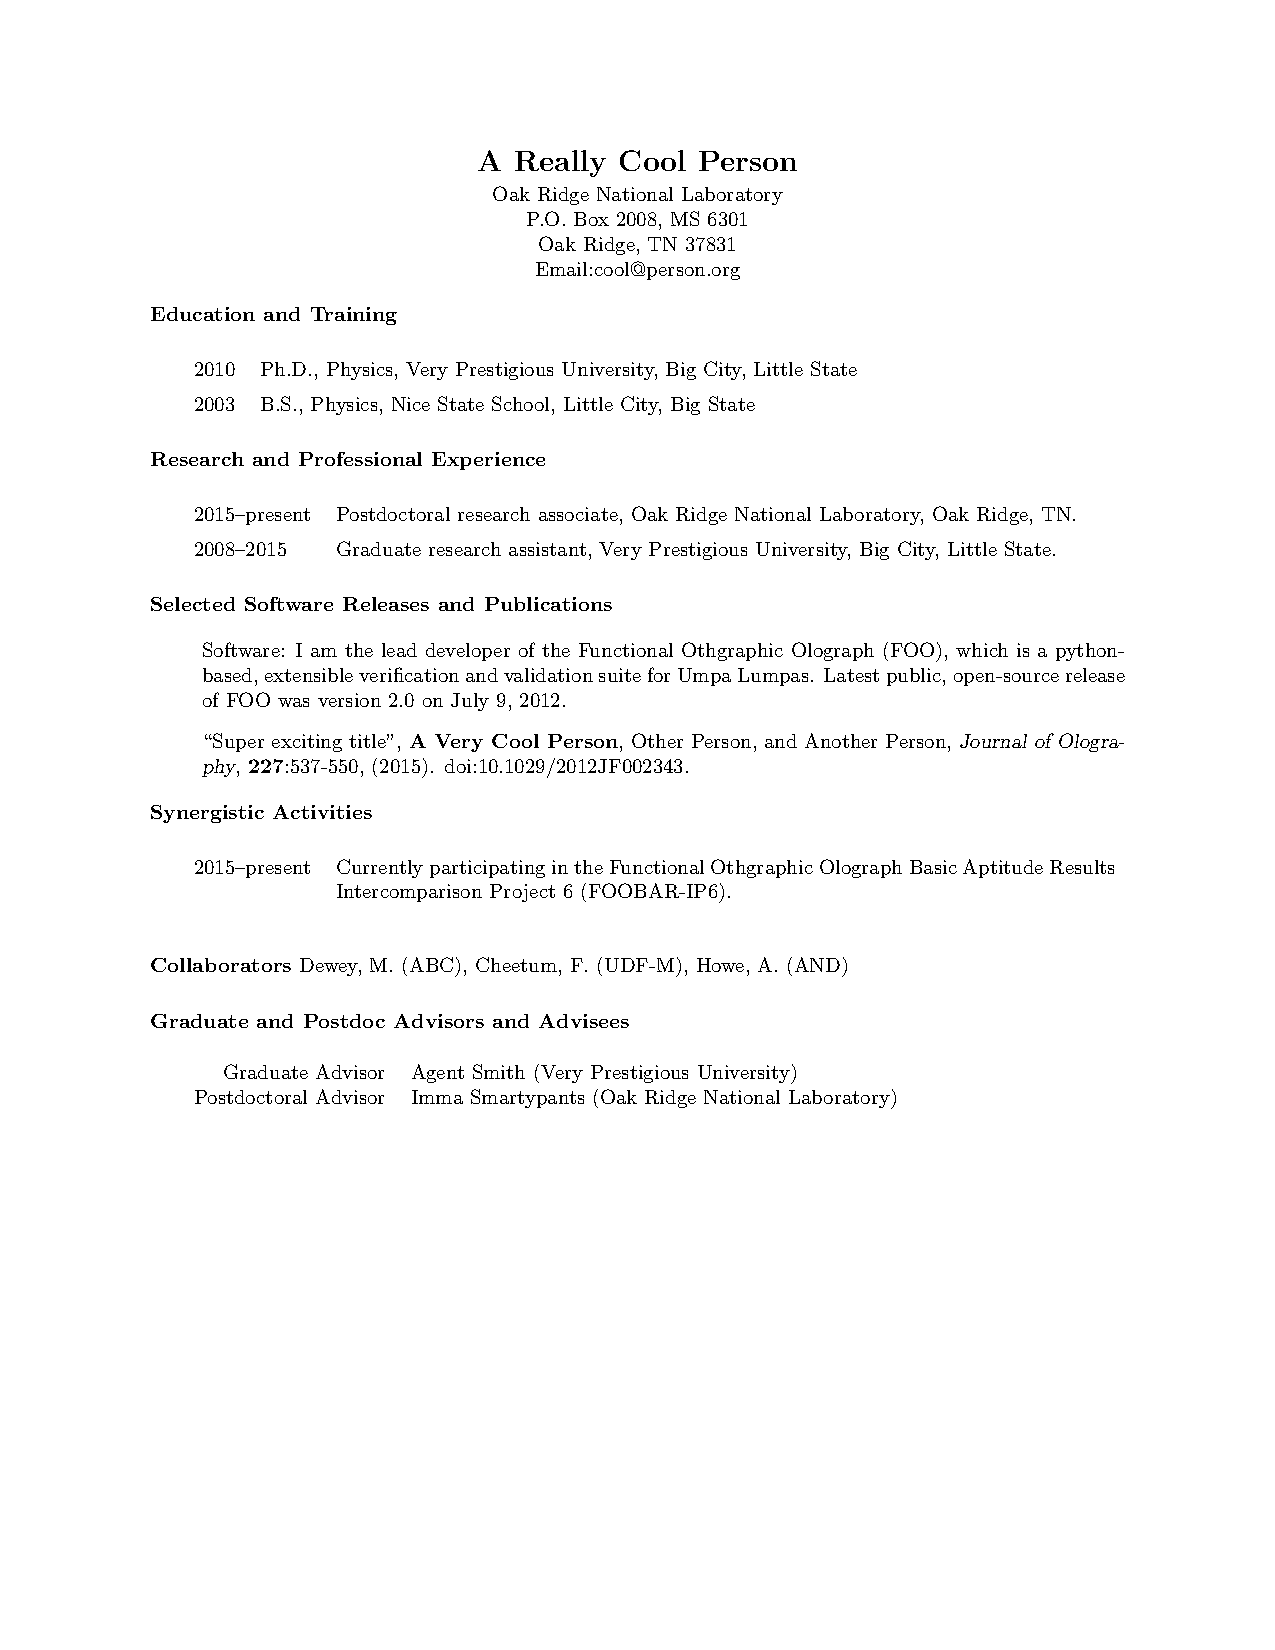
\includepdf[pages=-,pagecommand={\thispagestyle{plain}}]{Bios/cv_example.pdf}


    

\end{document}
%%%%%%%%%%%%%%%%%%%%%%%%%%%%%%%%%%%%%%%%%%%%%%%%%%%%%%%%%%%%%%%%%%%%%%%%%%%%%%%
% End the document
%%%%%%%%%%%%%%%%%%%%%%%%%%%%%%%%%%%%%%%%%%%%%%%%%%%%%%%%%%%%%%%%%%%%%%%%%%%%%%%

